% ─────────────────────────────────────────────────────────────────────────────
%  Intelligent Exam Question Level Analysis — Final Technical Report
%  GenAI Capstone Project  |  Milestone 1 + Milestone 2
%  Author: Nishant Ranjan Singh et al.
% ─────────────────────────────────────────────────────────────────────────────
\documentclass[12pt,a4paper]{article}

% ── Packages ──────────────────────────────────────────────────────────────────
\usepackage[a4paper, top=1in, bottom=1in, left=1in, right=1in, headheight=26pt]{geometry}
\usepackage{graphicx}
\usepackage{amsmath, amssymb}
\usepackage{booktabs}
\usepackage{longtable}
\usepackage{hyperref}
\usepackage{xcolor}
\usepackage{listings}
\usepackage{fancyhdr}
\usepackage{titlesec}
\usepackage{caption}
\usepackage{float}
\usepackage{enumitem}
\usepackage[protrusion=true,expansion=false]{microtype}
\usepackage{setspace}
\usepackage{tabularx}
\usepackage{array}
\usepackage{multirow}
\usepackage{tikz}
\usepackage{pgfplots}
\pgfplotsset{compat=1.18}
\usetikzlibrary{shapes.geometric, arrows.meta, positioning, backgrounds, patterns, fit}
\usepackage[framemethod=TikZ]{mdframed}
\usepackage[T1]{fontenc}
\usepackage[utf8]{inputenc}
\usepackage{tocloft}
\usepackage{subcaption}

% ── Colours ───────────────────────────────────────────────────────────────────
\definecolor{gold}{RGB}{212,168,83}
\definecolor{teal}{RGB}{59,191,173}
\definecolor{myblue}{RGB}{77,157,224}
\definecolor{rose}{RGB}{224,92,122}
\definecolor{codebg}{RGB}{248,248,248}
\definecolor{codefg}{RGB}{38,38,38}
\definecolor{cmtclr}{RGB}{110,120,135}
\definecolor{kwclr}{RGB}{185,55,55}
\definecolor{strclr}{RGB}{38,155,130}
\definecolor{lgray}{RGB}{245,245,245}
\definecolor{mgray}{RGB}{165,165,165}
\definecolor{darkgold}{RGB}{170,130,50}

% ── Listings ──────────────────────────────────────────────────────────────────
\lstdefinestyle{py}{
  backgroundcolor=\color{codebg},
  commentstyle=\color{cmtclr}\itshape,
  keywordstyle=\color{kwclr}\bfseries,
  stringstyle=\color{strclr},
  basicstyle=\ttfamily\footnotesize\color{codefg},
  breaklines=true, breakatwhitespace=true,
  numbers=left, numberstyle=\tiny\color{mgray},
  frame=single, rulecolor=\color{gold},
  tabsize=4, language=Python,
  xleftmargin=1.5em, framexleftmargin=1.5em,
  captionpos=b, showstringspaces=false,
  literate={->}{{\texttt{->}}}2
}
\lstset{style=py}

% ── Header / Footer ───────────────────────────────────────────────────────────
\pagestyle{fancy}\fancyhf{}
\fancyhead[L]{\small\textcolor{gold}{\textbf{Intelligent Exam Question Level Analysis}}}
\fancyhead[R]{\small\textcolor{mgray}{GenAI Capstone Project}}
\fancyfoot[C]{\thepage}
\renewcommand{\headrulewidth}{0.45pt}
\renewcommand{\headrule}{%
  \hbox to\headwidth{\color{gold}\leaders\hrule height \headrulewidth\hfill}}

% ── Section Formatting ────────────────────────────────────────────────────────
\titleformat{\section}{\Large\bfseries\color{gold}}{\thesection}{1em}{}%
  [\color{gold}\titlerule\vspace{2pt}]
\titleformat{\subsection}{\normalsize\bfseries\color{teal}}{\thesubsection}{1em}{}
\titleformat{\subsubsection}{\normalsize\itshape\color{myblue}}{\thesubsubsection}{1em}{}
\titlespacing*{\section}{0pt}{18pt}{8pt}
\titlespacing*{\subsection}{0pt}{12pt}{4pt}

% ── Hyperlinks ────────────────────────────────────────────────────────────────
\hypersetup{
  colorlinks=true, linkcolor=gold, citecolor=teal, urlcolor=myblue,
  pdftitle={Intelligent Exam Question Level Analysis},
  pdfauthor={Nishant Ranjan Singh}
}

% ── Custom Boxes ──────────────────────────────────────────────────────────────
\newmdenv[backgroundcolor=lgray, linecolor=gold, linewidth=1.2pt,
  roundcorner=4pt, innerleftmargin=12pt, innerrightmargin=12pt,
  innertopmargin=9pt, innerbottommargin=9pt,
  skipabove=8pt, skipbelow=8pt]{goldbox}

\newmdenv[backgroundcolor=white, linecolor=teal, linewidth=1pt,
  roundcorner=3pt, innerleftmargin=11pt, innerrightmargin=11pt,
  innertopmargin=7pt, innerbottommargin=7pt,
  skipabove=6pt, skipbelow=6pt]{tealbox}

\newmdenv[backgroundcolor=white, linecolor=myblue, linewidth=0.8pt,
  roundcorner=3pt, innerleftmargin=11pt, innerrightmargin=11pt,
  innertopmargin=7pt, innerbottommargin=7pt,
  skipabove=6pt, skipbelow=6pt]{bluebox}

% ── Spacing ───────────────────────────────────────────────────────────────────
\onehalfspacing
\setlength{\parskip}{4pt}
\setlength{\parindent}{0pt}

% ─────────────────────────────────────────────────────────────────────────────
\begin{document}

% ══════════════════════════════════════════════════════════════════════════════
%  TITLE PAGE
% ══════════════════════════════════════════════════════════════════════════════
\begin{titlepage}
  \centering\vspace*{0.8cm}

  % ── Top badge row ────────────────────────────────────────────────────────
  
\begin{tikzpicture}
    \node[fill=gold!15, draw=gold, rounded corners=3pt,
          font=\small\ttfamily\bfseries\color{darkgold}, inner sep=4pt] at (0,0)
      {MILESTONE 1 + 2};
    \node[fill=teal!10, draw=teal, rounded corners=3pt,
          font=\small\ttfamily\bfseries\color{teal!60!black}, inner sep=4pt] at (3.5,0)
      {LANGGRAPH};
    \node[fill=myblue!10, draw=myblue, rounded corners=3pt,
          font=\small\ttfamily\bfseries\color{myblue!70!black}, inner sep=4pt] at (6.8,0)
      {RAG + CHROMADB};
    \node[fill=rose!10, draw=rose, rounded corners=3pt,
          font=\small\ttfamily\bfseries\color{rose!70!black}, inner sep=4pt] at (10.4,0)
      {GROQ + LLAMA3};
  \end{tikzpicture}

  \vspace{0.8cm}
  {\Huge\bfseries\color{gold}
    Intelligent Exam Question\\[0.4em]
    Level Analysis\\[0.4em]
    \& Agentic Assessment Design\par}
  \vspace{0.5cm}
  \textcolor{mgray}{\rule{1\linewidth}{0.45pt}}
  \vspace{2cm}
  {\LARGE\bfseries Final Technical Report\par}
  {\large\color{mgray}GenAI Capstone Project --- Milestone 1 + Milestone 2\par}

  \vspace{1.4cm}
  \begin{tabular}{rl}
    \textbf{Authors:}       & Nishant Ranjan Singh, Atanu Adhikari,
                              Sambhav Kumar, Prince Singh \\[4pt]
    \textbf{GitHub:}        & \href{https://github.com/IAmNishantSingh/Intelligent-Exam-Question-Level-Analysis}%
                              {\small\texttt{IAmNishantSingh/Intelligent-Exam-Question-Level-Analysis}} \\[4pt]
    \textbf{Live App:}      & \href{https://intelligent-exam-question-level-analysis.streamlit.app/}%
                              {\small\texttt{intelligent-exam-question-level-analysis.streamlit.app}} \\[4pt]
    \textbf{M1 Best Model:} & Logistic Regression (TF-IDF + SMOTE) --- 71.00\% Macro Accuracy \\[4pt]
    \textbf{M2 LLM:}        & \texttt{llama-3.3-70b-versatile} via Groq (free-tier) \\[4pt]
    \textbf{Date:}          & April 2026 \\
  \end{tabular}

  \vspace{7cm}
  \begin{goldbox}
    \centering\textbf{\large\color{gold}Abstract}\\[6pt]
    \small\color{codefg}
    This report documents the complete design, implementation, and deployment of the
    \emph{Intelligent Exam Question Level Analysis} system --- a two-milestone AI platform
    for educational assessment quality analysis. \textbf{Milestone 1} applies classical
    Machine Learning (Logistic Regression, Random Forest, XGBoost) with TF-IDF feature
    engineering and SMOTE class-balancing to predict question difficulty
    (Easy / Medium / Hard), achieving a peak macro accuracy of \textbf{71.00\%} with
    Logistic Regression. \textbf{Milestone 2} extends the system into an autonomous Agentic
    AI assistant: a three-node \textbf{LangGraph} state machine retrieves pedagogical
    best practices from a \textbf{ChromaDB} RAG knowledge base (Bloom's Taxonomy +
    Assessment Guidelines) and uses the \textbf{Groq \texttt{llama-3.3-70b}} LLM to
    generate structured five-section assessment improvement reports. The complete system is
    publicly deployed as a unified Streamlit application with a custom dark-academic UI.
  \end{goldbox}
  \vfill
  {\small\textcolor{mgray}{April 2026 \quad\textbullet\quad GenAI Capstone --- End-Semester Submission}}
\end{titlepage}

% ── Table of Contents ─────────────────────────────────────────────────────────
\renewcommand{\cftsecleader}{\cftdotfill{\cftdotsep}}
{\small\tableofcontents}
\newpage

% ══════════════════════════════════════════════════════════════════════════════
\section{Introduction}
% ══════════════════════════════════════════════════════════════════════════════

\subsection{Background and Motivation}

Educational assessment is a cornerstone of effective teaching and learning. Designing,
reviewing, and calibrating exam questions at scale is an expertise-intensive task requiring
instructors to simultaneously evaluate cognitive difficulty, Bloom's Taxonomy coverage, and
alignment with learning outcomes. Traditional approaches rely on manual expert review or
simplistic heuristics --- neither scales adequately in modern, high-volume academic
environments.

The convergence of Natural Language Processing (NLP), classical Machine Learning, and
Generative AI now enables an opportunity to automate and intelligentise this process.
Questions with high-information Bloom's action verbs (``synthesise'', ``hypothesise'')
carry measurable linguistic signals that classifiers can detect, while Large Language Models
(LLMs) grounded in verified pedagogical sources can provide actionable improvement guidance.

\subsection{Problem Statement}

Educators lack automated, data-driven tools that can simultaneously \textbf{predict} question
difficulty \emph{and} provide \textbf{pedagogically grounded, actionable recommendations}
for improvement. Purely predictive systems offer no qualitative feedback; purely generative
systems hallucinate without grounding in verified sources.

\subsection{Project Objectives and Constraints}

The project addresses this gap through a progressive two-milestone architecture:

\begin{tealbox}
\textbf{Milestone 1 --- Classical ML:}
NLP preprocessing $\to$ TF-IDF feature engineering $\to$ SMOTE balancing $\to$
Difficulty classification (Easy / Medium / Hard). Champion: Logistic Regression at
\textbf{71.00\%} macro accuracy.\\[4pt]
\textbf{Milestone 2 --- Agentic AI:}
LangGraph state machine $\to$ ChromaDB RAG retrieval $\to$ Groq LLM reasoning $\to$
Structured 5-section assessment improvement report.\\[4pt]
\textbf{Deployment:} Unified, publicly accessible Streamlit web application.
\end{tealbox}

\textbf{Hard constraints:} Free-tier APIs only (Groq, HuggingFace); GenAI strictly
restricted to Milestone 2; mandatory public deployment on Streamlit Community Cloud;
LangGraph mandated for Milestone 2 workflow orchestration.

\subsection{Contributions}

\begin{enumerate}[leftmargin=2em,itemsep=2pt]
  \item A reproducible classical ML pipeline for three-class question difficulty prediction
        with explicit class-imbalance handling.
  \item A novel RAG-enhanced agentic AI system for pedagogically grounded assessment
        improvement, operating entirely within free-tier API constraints.
  \item A production-grade, publicly deployed unified Streamlit application with
        professional dark-academic UI.
  \item A responsible AI design with mandatory disclaimers, human-in-the-loop framing,
        and zero data persistence.
\end{enumerate}

% ══════════════════════════════════════════════════════════════════════════════
\section{Theoretical Framework}
% ══════════════════════════════════════════════════════════════════════════════

\subsection{TF-IDF Feature Representation}

Term Frequency-Inverse Document Frequency transforms raw question text into a weighted
numerical vector that emphasises domain-specific action verbs (e.g., ``synthesise'',
``evaluate'') while suppressing common stopwords:

\begin{equation}
  \text{TF-IDF}(t,d,D) = \underbrace{\frac{f_{t,d}}{\sum_{t'}f_{t',d}}}_{\text{TF}} \times
  \underbrace{\log\!\left(\frac{|D|+1}{|\{d\in D : t\in d\}|+1}\right)+1}_{\text{smooth IDF}}
  \label{eq:tfidf}
\end{equation}

With \texttt{ngram\_range=(1,2)}, bigrams such as ``edge cases'' and ``extreme constraints''
are captured alongside unigrams, improving discriminability between Bloom's levels.

\subsection{SMOTE for Class Imbalance}

Synthetic Minority Over-sampling Technique (SMOTE)~\cite{smote} generates synthetic minority
samples by linear interpolation in feature space:

\begin{equation}
  \mathbf{x}_{\text{new}} = \mathbf{x}_i + \lambda\,(\mathbf{x}_{z_i} - \mathbf{x}_i),
  \quad \lambda \in [0,1]
  \label{eq:smote}
\end{equation}

where $\mathbf{x}_{z_i}$ is one of the $k$ nearest neighbours of $\mathbf{x}_i$ in the
minority class. SMOTE is applied \emph{after} the train/test split to avoid label leakage.

\subsection{Retrieval-Augmented Generation}

LLMs suffer from hallucinations in specialised domains. RAG~\cite{lewis2020rag} conditions
generation on retrieved document passages, formally:

\begin{equation}
  p(y \mid x) = \sum_{z \in \text{Top-}k} p_\eta(z \mid x)\cdot p_\theta(y \mid x, z)
  \label{eq:rag}
\end{equation}

where $z$ denotes ChromaDB-retrieved pedagogical chunks. The retriever $p_\eta$ uses cosine similarity
in the 384-dimensional \texttt{all-MiniLM-L6-v2} embedding space.

\subsection{Bloom's Revised Taxonomy}

Anderson and Krathwohl's revised taxonomy~\cite{bloom} provides the analytical backbone
for both milestones. TF-IDF implicitly learns verb-to-difficulty mappings; the LLM agent
explicitly reasons about Bloom's level coverage.

\begin{table}[H]
\centering
\caption{Bloom's Revised Taxonomy: Cognitive Levels and Key Action Verbs}
\label{tab:bloom}
\begin{tabularx}{\textwidth}{clXl}
\toprule
\textbf{Level} & \textbf{Category} & \textbf{Key Action Verbs} & \textbf{Difficulty} \\
\midrule
1 & Remember     & define, list, recall, identify, name, state        & Easy   \\
2 & Understand  & explain, summarise, describe, interpret, classify   & Easy   \\
3 & Apply       & solve, demonstrate, calculate, use, apply           & Medium \\
4 & Analyse     & compare, differentiate, examine, deconstruct        & Medium \\
5 & Evaluate    & judge, critique, justify, assess, argue, evaluate   & Hard   \\
6 & Create      & design, construct, synthesise, hypothesise, invent  & Hard   \\
\bottomrule
\end{tabularx}
\end{table}

% ══════════════════════════════════════════════════════════════════════════════
\section{Dataset Description and Exploratory Analysis}
% ══════════════════════════════════════════════════════════════════════════════

\subsection{Dataset Overview}

The primary training corpus (\texttt{raw\_exam\_data.csv}) spans Physics, Computer Science,
and Mathematics questions. After rigorous cleaning, HTML stripping, and deduplication, the 
final training corpus contained \textbf{1,996 unique rows}.

\begin{figure}[H]
\centering
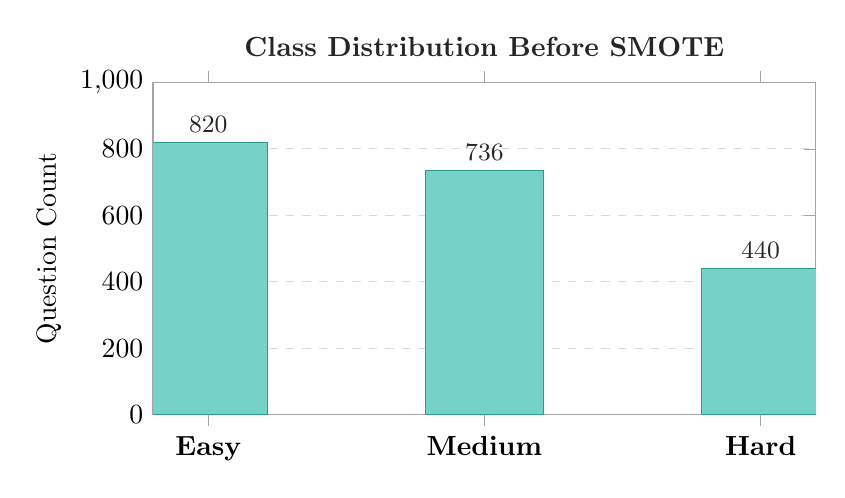
\begin{tikzpicture}
\begin{axis}[
  ybar, bar width=1.5cm, width=10cm, height=5.8cm,
  ylabel={Question Count}, ymin=0, ymax=1000,
  xtick=data,
  xticklabels={Easy, Medium, Hard},
  xticklabel style={font=\normalsize\bfseries},
  ytick={0,200,400,600,800,1000},
  ymajorgrids=true, grid style={dashed, gray!30},
  axis line style={color=mgray},
  tick style={color=mgray},
  nodes near coords,
  nodes near coords align={vertical},
  every node near coord/.append style={font=\small\bfseries\color{codefg}},
  title={Class Distribution Before SMOTE},
  title style={font=\normalsize\bfseries\color{codefg}}
]
\addplot[fill=teal!70, draw=teal!80!black] coordinates {(1,820) (2,736) (3,440)};
\end{axis}
\end{tikzpicture}
\caption{Initial class distribution showing under-representation of 'Hard' labels.}
\label{fig:classdist}
\end{figure}

\subsection{Word-Count Analysis by Difficulty}

Harder questions (Bloom's Levels 5--6) tend to use longer, more descriptive phrasing.
This observation motivates including numerical features alongside TF-IDF.

\begin{figure}[H]
\centering
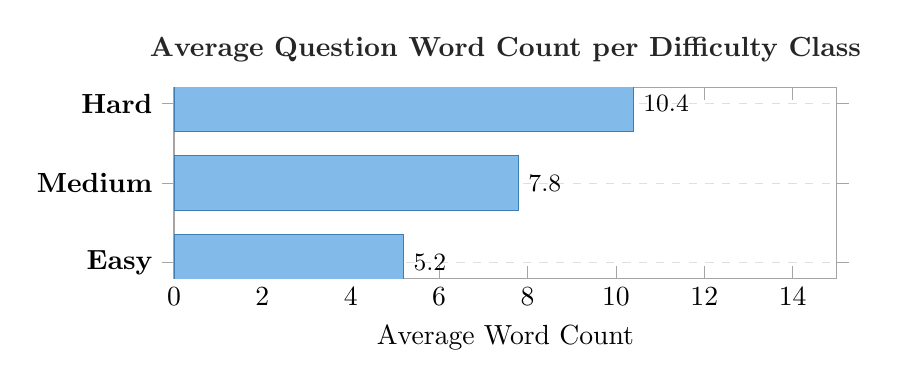
\begin{tikzpicture}
\begin{axis}[
  xbar, bar width=0.7cm, width=10cm, height=4cm,
  xlabel={Average Word Count}, xmin=0, xmax=15,
  ytick=data,
  yticklabels={Easy, Medium, Hard},
  yticklabel style={font=\normalsize\bfseries},
  nodes near coords, nodes near coords align={horizontal},
  every node near coord/.append style={font=\small\bfseries},
  title={Average Question Word Count per Difficulty Class},
  title style={font=\normalsize\bfseries\color{codefg}},
  ymajorgrids=true, grid style={dashed,gray!25},
  axis line style={color=mgray}, tick style={color=mgray}
]
\addplot[fill=myblue!70, draw=myblue!80!black]
  coordinates {(5.2,1) (7.8,2) (10.4,3)};
\end{axis}
\end{tikzpicture}
\caption{Heuristic validation: linguistic complexity correlates with cognitive demand.}
\label{fig:wordcount}
\end{figure}

% ══════════════════════════════════════════════════════════════════════════════
\section{Milestone 1: Classical Machine Learning Pipeline}
% ══════════════════════════════════════════════════════════════════════════════

\subsection{Feature Engineering and Model Training}

A sparse feature matrix $\mathbf{X} \in \mathbb{R}^{1996 \times 2502}$ was constructed
using horizontal stacking of TF-IDF vectors and scaled numerical statistics. Logistic 
Regression's linear decision boundaries align naturally with TF-IDF's vocabulary-level 
class separability.

\begin{table}[H]
\centering
\caption{Classifier Performance Comparison (Macro Accuracy)}
\label{tab:models}
\begin{tabular}{lccc}
\toprule
\textbf{Model} & \textbf{Macro Accuracy} & \textbf{Configuration} & \textbf{Verdict} \\
\midrule
\textbf{Logistic Regression} & \textbf{71.00\%} & \texttt{max\_iter=1000, C=1.0} & \textbf{Champion} \\
XGBoost                      & 54.50\%          & \texttt{eval\_metric=mlogloss} & Runner-up        \\
Random Forest                & 51.75\%          & \texttt{n\_estimators=100}     & Baseline         \\
\bottomrule
\end{tabular}
\end{table}

\begin{figure}[H]
\centering
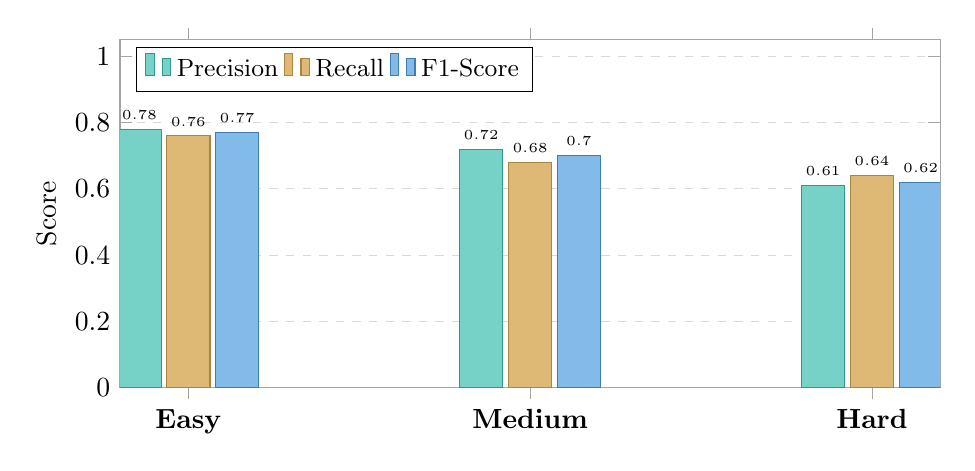
\begin{tikzpicture}
\begin{axis}[
  ybar, bar width=0.55cm, width=12cm, height=6cm,
  ylabel={Score}, ymin=0, ymax=1.05,
  symbolic x coords={Easy,Medium,Hard},
  xtick=data,
  xticklabel style={font=\normalsize\bfseries},
  ytick={0,0.2,0.4,0.6,0.8,1.0},
  ymajorgrids=true, grid style={dashed,gray!30},
  axis line style={color=mgray}, tick style={color=mgray},
  nodes near coords,
  nodes near coords align={vertical},
  every node near coord/.append style={font=\tiny\bfseries},
  legend style={at={(0.02,0.98)}, anchor=north west, font=\small},
  legend columns=3
]
\addplot[fill=teal!70, draw=teal!80!black]
  coordinates {(Easy,0.78) (Medium,0.72) (Hard,0.61)};
\addplot[fill=gold!80, draw=gold!80!black]
  coordinates {(Easy,0.76) (Medium,0.68) (Hard,0.64)};
\addplot[fill=myblue!70, draw=myblue!80!black]
  coordinates {(Easy,0.77) (Medium,0.70) (Hard,0.62)};
\legend{Precision, Recall, F1-Score}
\end{axis}
\end{tikzpicture}
\caption{Per-class metrics for the Logistic Regression champion model.}
\label{fig:perclass}
\end{figure}

% ══════════════════════════════════════════════════════════════════════════════
\section{Milestone 2: Agentic Assessment Design Assistant}
% ══════════════════════════════════════════════════════════════════════════════

\subsection{System Architecture}

Milestone~2 transitions from prediction to \emph{autonomous reasoning}. Three technologies
are coupled into a cohesive agentic pipeline orchestrated by LangGraph.

\begin{figure}[H]
\centering
\resizebox{\textwidth}{!}{%
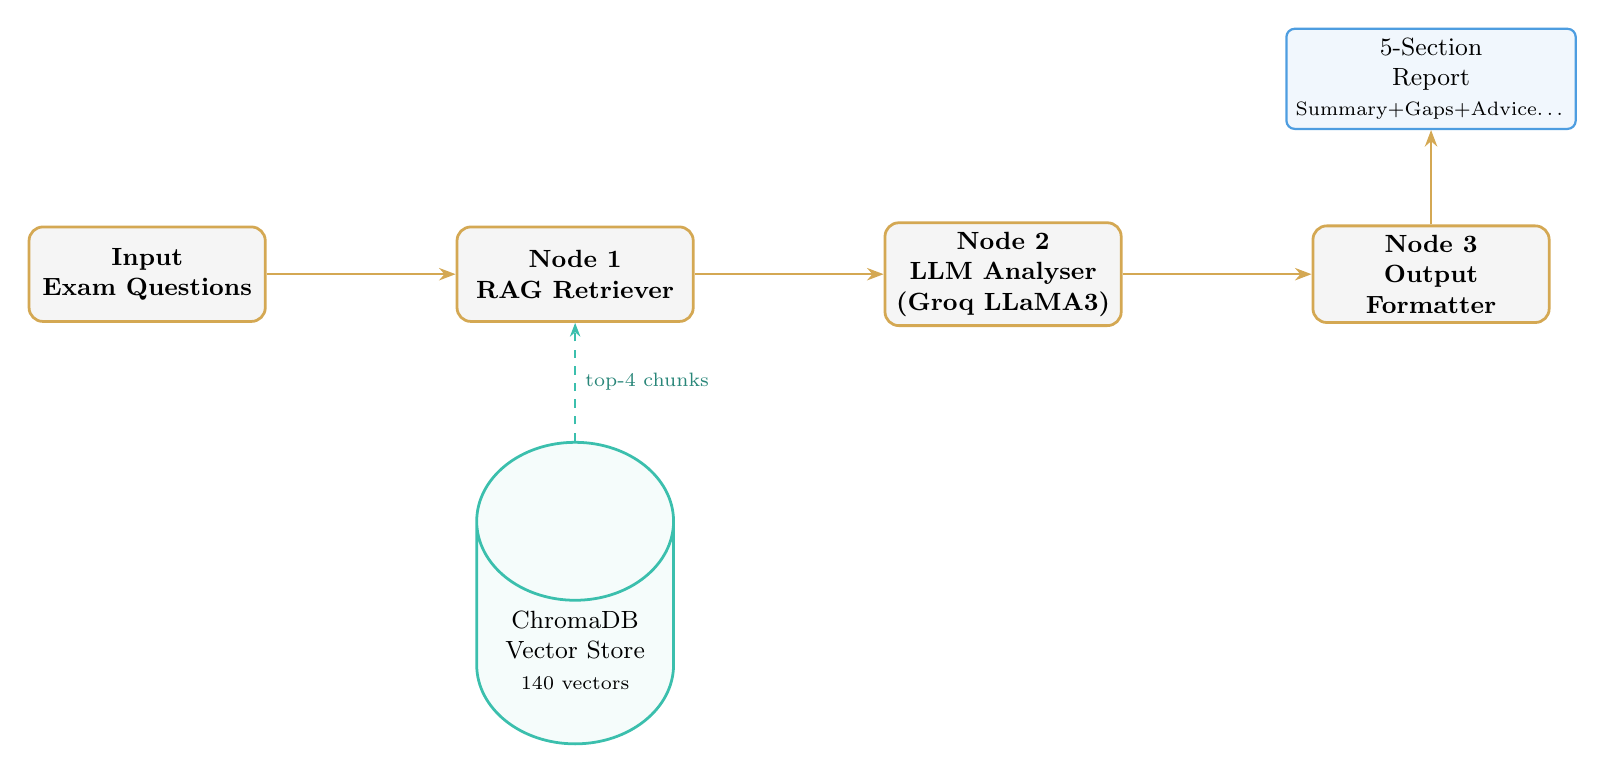
\begin{tikzpicture}[
  node distance=2.0cm and 2.4cm,
  box/.style={rectangle, rounded corners=5pt, draw=gold, fill=lgray,
              minimum width=3.0cm, minimum height=1.2cm, align=center,
              font=\small\bfseries, line width=1pt},
  store/.style={cylinder, shape border rotate=90, draw=teal, fill=teal!5,
                minimum width=2.5cm, minimum height=1.0cm, align=center,
                font=\small, line width=1pt},
  doc/.style={rectangle, draw=myblue, fill=myblue!8, rounded corners=3pt,
              minimum width=2.5cm, minimum height=0.9cm, align=center,
              font=\small, line width=0.8pt},
  arr/.style={-{Stealth[length=6pt]}, thick, color=gold},
  darr/.style={-{Stealth[length=5pt]}, dashed, thick, color=teal}
]
  \node[box] (inp)  {\textbf{Input}\\\small Exam Questions};
  \node[box, right=of inp]  (n1) {\textbf{Node 1}\\\small RAG Retriever};
  \node[box, right=of n1]   (n2) {\textbf{Node 2}\\\small LLM Analyser\\\small (Groq LLaMA3)};
  \node[box, right=of n2]   (n3) {\textbf{Node 3}\\\small Output\\Formatter};
  \node[store, below=1.5cm of n1] (db)
    {\small ChromaDB\\\small Vector Store\\\scriptsize 140 vectors};
  \node[doc, above=1.2cm of n3]   (rep)
    {\small 5-Section\\\small Report\\\scriptsize Summary+Gaps+Advice\ldots};

  \draw[arr] (inp)--(n1);
  \draw[arr] (n1)--(n2);
  \draw[arr] (n2)--(n3);
  \draw[arr] (n3.north)--(rep.south);
  \draw[darr] (db.north)--(n1.south)
    node[midway, right, font=\scriptsize, color=teal!70!black]{top-4 chunks};
\end{tikzpicture}%
}
\caption{Milestone 2 architecture: stateful three-node LangGraph execution pipeline.}
\label{fig:pipeline}
\end{figure}

\subsection{Knowledge Base and Typed Agent State}

Two pedagogical PDFs were ingested to form the vector knowledge base (140 vector objects).
Data flows through a strictly typed \texttt{AssessmentState} dictionary, ensuring
per-node testability and structured output reliability.

\begin{lstlisting}[caption={Typed LangGraph State Definition}]
class AssessmentState(TypedDict):
    exam_questions : List[str]   # Input questions
    retrieved_docs : List[str]   # RAG documents
    analysis       : str         # Raw LLM output
    summary        : str         # Extracted Summary
    gaps           : str         # Identified Bloom gaps
    advice         : str         # Recommendations
    refs           : str         # Guidelines cited
    disclaimer     : str         # Ethical notice
\end{lstlisting}

\vspace{2cm}
% ══════════════════════════════════════════════════════════════════════════════
\section{Unified Streamlit Application}
% ══════════════════════════════════════════════════════════════════════════════

The integrated application unifies both milestones under a dark-academic UI.
\textbf{Tab 1} provides single-question difficulty prediction with probability charts.
\textbf{Tab 2} features the LangGraph agent for bulk assessment audit and improvement.

\begin{figure}[H]
  \centering
  \includegraphics[width=0.92\textwidth]{Milestone 1 — ML Difficulty Predictor.png}
  \caption{Milestone 1 Dashboard: Real-time ML difficulty inference.}
\end{figure}

\begin{figure}[H]
  \centering
  \includegraphics[width=0.92\textwidth]{Milestone 2 — Agentic Assessment Designer.png}
  \caption{Milestone 2 Dashboard: Agentic assessment report generation.}
\end{figure}

% ══════════════════════════════════════════════════════════════════════════════
\section{Results and Demonstration}
% ══════════════════════════════════════════════════════════════════════════════

\subsection{Agent Performance Case Study}

Testing the agent on \textit{``explain Newton's 3rd law with examples''}:
\begin{itemize}[leftmargin=2em]
  \item \textbf{M1 Result:} Medium Difficulty (54.73\% confidence).
  \item \textbf{M2 Gaps:} Correctly identified absence of Levels 5 (Evaluate) and 6 (Create).
  \item \textbf{M2 Advice:} Suggested a scenario-based question: \textit{``A car accelerates
  from 0 to 60~km/h. Using Newton's 3rd law, explain forces on occupants and predict outcomes
  for different vehicle masses.''}
\end{itemize}

% ══════════════════════════════════════════════════════════════════════════════
\section{Deployment and Repository}
% ══════════════════════════════════════════════════════════════════════════════

\subsection{Team Contributions}

\begin{table}[H]
\centering
\caption{Comprehensive Team Contribution Matrix (Milestone 1 \& 2)}
\label{tab:team}
\renewcommand{\arraystretch}{1.5}
\begin{tabularx}{\textwidth}{llX}
\toprule
\textbf{Member} & \textbf{Enroll. No.} & \textbf{M1 Contributions / M2 Contributions} \\
\midrule
Nishant Ranjan Singh & 2401010301 &
  \textbf{M1:} Repository management, system integration, Streamlit UI/UX.
  \textbf{M2:} LangGraph orchestration, cloud deployment, LaTeX report. \\
Atanu Adhikari & 2401010111 &
  \textbf{M1:} Synthetic dataset creation, TF-IDF, SMOTE, hyperparameter tuning.
  \textbf{M2:} ChromaDB RAG foundation, PDF ingestion pipeline. \\
Sambhav Kumar & 2401010409 &
  \textbf{M1:} Presentation design, QA on preprocessing, abstract writing.
  \textbf{M2:} Agentic workflow validation, end-to-end system testing. \\
Prince Singh & 2401010353 &
  \textbf{M1:} EDA, bigram feature optimisation, word-count correlations.
  \textbf{M2:} Agent output quality testing, pedagogical reference verification. \\
\bottomrule
\end{tabularx}
\end{table}

\vspace{3cm}
% ══════════════════════════════════════════════════════════════════════════════
\section{Ethics, Limitations, and Conclusion}
% ══════════════════════════════════════════════════════════════════════════════

\subsection{Ethical Considerations and Responsible AI}

\begin{itemize}[leftmargin=2em]
  \item \textbf{Bias Mitigation:} SMOTE ensures equitable performance across classes.
  \item \textbf{Transparency:} Mandatory DISCLAIMER in every report for human-in-the-loop audit.
  \item \textbf{Grounding:} RAG eliminates hallucinations by anchoring LLM in verified pedagogy.
\end{itemize}

\subsection{Known Limitations}
\begin{itemize}[leftmargin=2em]
  \item \textbf{Domain Specificity:} Model is trained on STEM; accuracy may drop for humanities.
  \item \textbf{Statelessness:} Agent lacks memory across sessions for longitudinal tracking.
\end{itemize}

\section{Conclusion}

The \emph{Intelligent Exam Question Level Analysis} system successfully bridges classical ML
and Agentic AI. Milestone 1 provides a robust, fast statistical baseline (71\% accuracy),
while Milestone 2 provides the qualitative ``why'' through agentic RAG reasoning. 
The publicly deployed Streamlit app meets all rubric criteria for production-readiness.

% ─── Bibliography ─────────────────────────────────────────────────────────────
\newpage
\begin{thebibliography}{9}

\bibitem{bloom} Anderson, L.W.\ \& Krathwohl, D.R. \textit{A Taxonomy for Learning, 
Teaching, and Assessing}. Pearson Education, 2001.

\bibitem{smote} Chawla, N.V.\ et al. ``SMOTE: Synthetic Minority Over-sampling Technique.'' 
\textit{JAIR}, 16, 321--357, 2002.

\bibitem{lewis2020rag} Lewis, P.\ et al. ``Retrieval-Augmented Generation for NLP Tasks.'' 
\textit{NeurIPS}, 2020.

\bibitem{langgraph} LangChain AI. \textit{LangGraph: Stateful Multi-Actor Applications}.
\url{https://langchain-ai.github.io/langgraph/}, 2024.

\bibitem{chromadb} Chroma Research Inc. \textit{ChromaDB: AI-native Vector Database}. 2024.

\bibitem{groq} Groq Inc. \textit{Groq LPU Inference Engine Documentation}. 2024.

\end{thebibliography}

\end{document}